% !TEX root = ../notes.tex

\section{Introduction}

In this module we are going to consider continuous time models under the pretense of biological systems,
$$ \di x t = f(x, t, \mu) $$

\begin{eg}
  Here's an example we will use a couple of times,
  $$ \di N t = f(N, t, \vec \mu) = rN \left( 1 - \frac{N}{K} \right) $$
  where $\vec\mu = \begin{pmatrix}
    r \\ K
  \end{pmatrix}$
\end{eg}

We are also going to look at discrete systems, these are going to be through difference equations.
$$ \vec x (t + 1) = A\vec x(t) $$

and also we shall study PDEs,

$$ \pd u t = f(x, t, x, \mu, \pd u x, \pdd u x) $$

\begin{eg}
  $$ \pd u t = Ku(1 - u) + D\pdd u x $$
\end{eg}


\section{Continuous Models for a single species}
We are going to model simply how we model population dynamics for a single species. We are going to call $N(t)$ our population size at a certain time. We are going to say that $N(t)$ is continuous. We also say $N \in \R$ and so it's going to be a density measure. We are going to constrain this $N \ge 0, \,\fa t$. We can measure this and create a model,
$$ \di N t = f(N, t, \vec \mu) $$
We call $N$ the variable, then $\vec \mu$ the parameter. We let $t \in \R$ and $t > 0$. \\

Let's start off by thinking about an actual population of individuals, we have observed that there is some sort of growth dynamics. We can write a mechanistic model, by including mechanisms that affect the population.
$$ \di N t =  + \text{births} + \text{resources} + \text{net migration} - \text{deaths}  $$
If the positive things are greater, the population will grow, otherwise if they are smaller they decline, or they stay equal. \\

Now we make some assumptions, so we can write down a mathematical model.
\begin{enumerate}
  \item Births and deaths predominate:
  $$ \di N t = \text{births} - \text{deaths} $$
  \item Births and deaths are proportional to $N$:
  $$ \di N t = \a N - \b N \qquad \a, \b \in \R^{+}$$
  where we call $\a$ the birthrate and $\b$ the deathrate and $\vec \mu = (\a, \b)$.
\end{enumerate}

\begin{tcolorbox}

  If we consider, as an aside,
  $$ \di N t = \a N - \b N + \g \qquad \g \in \R $$
  this adds something like independent migration, where we assume migration is constant, this could be $\g N$ if it's proportional to $N$.

\end{tcolorbox}

We can solve this equation nicely,
\begin{align*}
  \di N t &= N(\a  - \b)\\
  \int \frac{1}{N}\di N t \,dt &= \int (\a - \b) dt\\
  \ln N &= (\a - \b)t + C \\
  N(t) &= Ae^{(\a - \b)t}
\end{align*}

Now assume this is an initial value problem, $N_0 = A$ and so,
$$ N(t) = N_0e^{(\a - \b)t} $$
We are also interested in the long term dynamics of these models, the asymptotic dynamics. Hence, we consider $t \to \infty$.
$$ \lim_{t \to \infty} N(t) = \begin{cases}
  \infty & \text{if $\a  > \b$}\\
  0 & \text{if $\a < \b$}\\
  N_0 & \text{ if $\a = \b$}
\end{cases} $$
We call the case where $\a = \b$ a steady state solution.\\


You don't usually see just a $t$ in the equation, but we may want to use a forcing term, i.e. periodic migration in Cornwall.
$$ \di N t = \a N - \b N + \cos (t) $$
We are not going to consider these non-autonomous systems. Hence we can write,
$$ \di N t = f(N, \vec \mu) $$
We have a nice thing to make sure our growth doesn't go exponential. It's the logistic map,
$$ \di N t = rN\left( 1 - \frac{N}{k} \right) \qquad r, k > 0 \quad N \ge 0 $$
where $f(N) = rN\left( 1 - \frac{N}{k} \right)$ is called the logistic model. This model has a level of self regulation, so if $N$ is high, then it will decrease later. Firstly, look at $f(N)$,
$$ f(N) = rN\left( 1 - \frac{N}{k}\right) $$
We start by graphing it,

\begin{figure}[!ht]
\centering
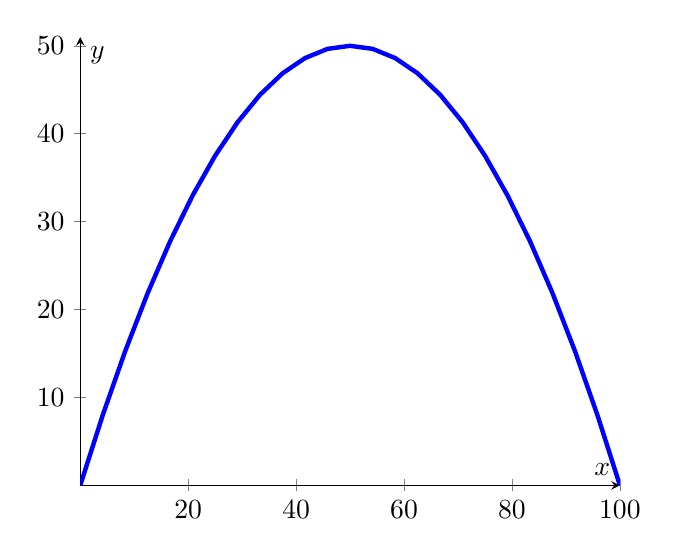
\begin{tikzpicture}[scale=1.0]
\begin{axis}[
        axis x line=middle,
        axis y line=middle,
        ymax=51, ylabel=$y$,
        xlabel=$x$
        ]
    \addplot[domain=0:100, blue, ultra thick] {2*x * (1 - x / 100)};
\end{axis}
\end{tikzpicture}
\caption{$y = 2x \left( 1 - \frac{x}{100}\right)$}
\end{figure}

\begin{exercise}
  Solve $\di N t = rN(1 - \frac{N}{k})$
\end{exercise}
The solution to this equation is,
$$ N(t) = \frac{N_0 k e^{rt}}{k - N_0 + N_0e^{rt}} $$

As $t \to \infty$, we can consider it and see that it will depend on $N_0$. If $N_0 = 0$, then we get that $N(t) = 0, \fa t$. If we then take $N_0 > 0$, then we get,
\begin{align*}
  N(t) &= \frac{N_0 k}{\frac{k - N_0}{e^{kt}} + N_0}\\
  &= k && t \to \infty
\end{align*}
